
\begin{figure}[h!]
\centering
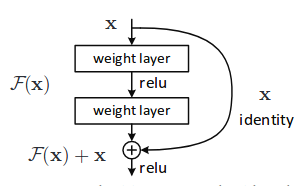
\includegraphics[scale=0.55]{pictures/residualBlock}
\caption{An diagram of a residual block. The input, $\vec{x}$, skips forward and is added to the ouput of the final convolutional layer \cite{ResNet}}
\label{fig:ResBlock}
\end{figure}

Since the residual CNN built by He et al. \cite{ResNet} won first place in the ILSVRC 2015 competition, residual blocks have been widely used to improve the performance of CNNs. Residual blocks have the output of an earlier convolutional block added with the output of a later one. Residual blocks are a solution to a problem of deep CNNs, which can perform worse than shallower ones. 

Suppose that we have a n-layered convolutional network, which takes as input some $\vec{x}$, produces an output $F(\vec{x})$ and tries to approximate some unknown function $H(\vec{x})$. If we add a new layer to the end of this network, which takes as input the previous output $F(\vec{x})$ and produces an output $G(F(\vec{x}))$, this new network should always be able to perform at least as well as the previous one by setting $G(F(\vec{x})) = F(\vec{x})$. This amounts to learning a weight matrix with a 1 in the middle and 0s elsewhere, such that the inputs are just copied over to the outputs. Therefore larger networks should always be able to perform at least as well as shallower ones, and therefore the reason for deeper networks being outperformed by shallower ones must be that this weight matrix is too difficult to learn. 

Residual blocks change this (see fig\ref{fig:ResBlock}). Instead of the block taking input $\vec{x}$, producing $F(\vec{x})$ and trying to approximate some $H(\vec{x})$ such that $F(\vec{x})\approx H(\vec{x})$, the block now produces $F(\vec{x}) + \vec{x}$ and thus tries to learn that $F(\vec{x}) \approx H(\vec{x}) - \vec{x}$ (see fig.\ref{fig:ResBlock}). The idea behind this is that if this block has nothing to learn, (i.e. $H(\vec{x}) = \vec{x}$) it should easily by able to set $F(\vec{x}) \equiv 0$. The relu activation function used in the convolutional layers means that this amounts to setting all weights to any negative value, which is much easier for the network to learn than the weight matrix in the non-residual case. Thus deeper networks should now easily be able to perform at least as well as their shallower counterparts. This proves to be the case, with deeper networks outperforming their shallower counterparts \cite{ResNet}.